\documentclass{article}

\title{Assignment 2}
\date{22nd September 2018}
\author{Siddharth Nayak EE16B073}
\usepackage{graphicx}
\usepackage{hyperref}
\usepackage{amsmath}
\usepackage{amsfonts}
\usepackage{amssymb}
\usepackage{geometry}
\usepackage{listings}
\usepackage{color}
\usepackage[colorinlistoftodos]{todonotes}
\usepackage[section]{placeins}
\usepackage[subsection]{placeins}
\geometry{legalpaper, portrait, margin=1in}
\newcommand\tab[1][1cm]{\hspace*{#1}}
\newcommand \Mycomb[2][^n]{\prescript{#1\mkern-0.5mu}{}C_{#2}}

 \hypersetup{
    colorlinks=true,
    linkcolor=blue,
    filecolor=magenta,      
    urlcolor=blue,
}
 
\urlstyle{same}
 
\begin{document}

\maketitle

\pagenumbering{arabic}

%%%%%%%%%%%%%%%%%%%%%%%%%%%%%%%%%%%%%%%%%%%%%%%%%%%%%%%%%%%%%%%%%%%%%%%%%%%%%%%%%%%%%%%%%%%%%%%%%%%%%%%%%%%%%%%%%%%%%%
\section{Taxi Driver Dilemma}
The given problem can be modelled as a DP problem with 'N' stages.\\
States $\rightarrow \{A,B,C\}$\\
Actions $\rightarrow 
\begin{cases}
0:\textrm{Cruise the streets looking for a passenger.}\\
1:\textrm{Go to the nearest taxi stand and wait in line.}\\
2:\textrm{Wait for a call from the dispatcher (this is not possible in town B because of poor reception).}
\end{cases}
$\\
The transition probabilities and the single stage rewards are given in the form of a matrix.\\
We have to find the optimal actions for number of stages N=10 and N=20.\\

\subsection{Case 1: N=10}
Setting the value of N=10 in the program we get the following results:\\

 \[
\begin{bmatrix}
    A      &  B &  C  \\
    1       & 1 & 1  \\
    1       & 1 & 1  \\
    1       & 1 & 1  \\
    1       & 1 & 1  \\
    1       & 1 & 1  \\
    1       & 1 & 1  \\
    1       & 1 & 1  \\
    1       & 1 & 1  \\
    0       & 1 & 1  \\
    0       & 0 & 0
\end{bmatrix}
\]
\\
In the above matrix each column represents the optimal action to be taken in that state. So the above matrix shows us that it is optimal to take the action '0': where the driver goes and waits at the nearest taxi stand and wait in line at each stage except the last stage where it is optimal to take action '1': which is cruise the streets and look for a passenger. Also in the second last stage we have action '0'  if in state 'A'.
\[
\begin{bmatrix}
A   &  B   &   C\\
123.01 & 136.85& 124.19\\
109.67& 123.50& 110.84\\
 96.32& 110.16& 97.50\\
 82.98& 96.81& 84.16\\
 69.63& 83.47& 70.81\\
 56.29& 70.12& 57.47\\
 42.96& 56.77& 44.13\\
 29.66& 43.42& 30.90\\
 17.75& 29.93& 17.87\\
 8&16& 7\\
 0& 0& 0
\end{bmatrix}
\]\\
In the above matrix the expected costs are printed for each stage and each state.\\

\subsection{Case 2: N=20}
Setting the value of N=20 in the program we get the following results:\\

 \[
\begin{bmatrix}
    A      &  B &  C  \\
    1       & 1 & 1  \\
    1       & 1 & 1  \\
    1       & 1 & 1  \\
    1       & 1 & 1  \\
    1       & 1 & 1  \\
    1       & 1 & 1  \\
    1       & 1 & 1  \\
    1       & 1 & 1  \\
    1       & 1 & 1  \\
    1       & 1 & 1  \\
    1       & 1 & 1  \\
    1       & 1 & 1  \\
    1       & 1 & 1  \\
    1       & 1 & 1  \\
    1       & 1 & 1  \\
    1       & 1 & 1  \\
    1       & 1 & 1  \\
    1       & 1 & 1  \\
    0       & 1 & 1  \\
    0       & 0 & 0
\end{bmatrix}
\]
\\
In the above matrix each column represents the optimal action to be taken in that state. So the above matrix shows us that it is optimal to take the action '0': where the driver goes and waits at the nearest taxi stand and wait in line at each stage except the last stage where it is optimal to take action '1': which is cruise the streets and look for a passenger. Also in the second last stage we have action '0'  if in state 'A'.
\[
\begin{bmatrix}
A   &  B   &   C\\
256.46& 270.29& 257.63\\
243.11& 256.95& 244.29\\
229.77& 243.60& 230.95\\
216.42& 230.26& 217.60\\
203.08& 216.91& 204.26\\
189.73& 203.57& 190.91\\
176.39& 190.22& 177.57\\
163.05& 176.88& 164.22\\
149.70& 163.53& 150.88\\
136.36& 150.19& 137.53\\
123.01 & 136.85& 124.19\\
109.67& 123.50& 110.84\\
 96.32& 110.16& 97.50\\
 82.98& 96.81& 84.16\\
 69.63& 83.47& 70.81\\
 56.29& 70.12& 57.47\\
 42.96& 56.77& 44.13\\
 29.66& 43.42& 30.90\\
 17.75& 29.93& 17.87\\
 8&16& 7\\
 0& 0& 0
\end{bmatrix}
\]\\
In the above matrix the expected costs are printed for each stage and each state.\\

If the driver chooses to take action '1':where the driver goes and waits at the nearest taxi stand and wait in line at each stage then it is not optimal as in the last stage, in the optimal actions we have to take action '0'.Also in the second last stage in state 'A' we have to take action '0'. Therefore it is not optimal to just take action'1' always in all stages.Also it makes sense to search for a passenger instead of waiting for a passenger at the last stage.\\

%%%%%%%%%%%%%%%%%%%%%%%%%%%%%%%%%%%%%%%%%%%%%%%%%%%%%%%%%%%%%%%%%%%%%%%%%%%%%%%%%%%%%%%%%%%%%%%%%%%%%%%%%%%%%%%%%%%%%%
\section{Gridworld}
In the given problem we have a gridworld with a 10x10 state-space.There are two goals: Goal 1 and Goal 2. In one case the Terminal state is Goal 1 and in another case we have the terminal state as Goal 2.\\
This problem can be modelled as a Stochastic Shortest Path Problem(SSP) with the terminal state being the goal state.\\
Actions $\rightarrow \{\textrm{up,right,down,left}\}$\\
As the transitions are stochastic in nature we have to apply the 'T' operator to get the optimal actions(policy) and the optimal cost for each of the states and available actions.\\


\subsection{When to stop?}
So the value iteration loop can go on till infinity. So we have to decide when to stop. This decision can be made with the help of the graph of $\delta_i=max(|J_{i+1}-J_{i}|)$ vs the number of iterations.\\
 So we can decide a particular threshold for $\delta_i (=0.01)$ so that if it's value reduces below that then we can stop the iterations as it would have converged.
 

\subsection{Plot of $\delta_i=max(|J_{i+1}-J_{i}|)$ vs the number of iterations}
The graph of $\delta_i$ vs the number of iterations has an exponential decrease which is consistent with the fact proved in the class that the value iteration(Repeated application of the 'T' operator) has an geometric decrease. 

\subsubsection{Goal 1:}
  \begin{figure}[h]
 \centering
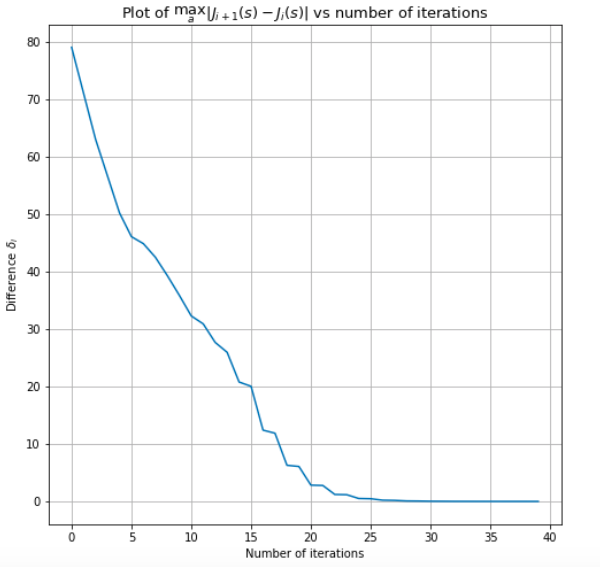
\includegraphics[width=8cm]{J1.png}
\caption{$\max(|J_{i+1}-J_{i}|)$ vs the number of iterations.}
\end{figure}\\
The value of $\delta_i$ goes below the value of 0.01 after 33 iterations. Thus it is ideal to stop the loop after 33 iterations as we have a converged value.

 \subsubsection{Goal 2:}
  \begin{figure}[h]
 \centering
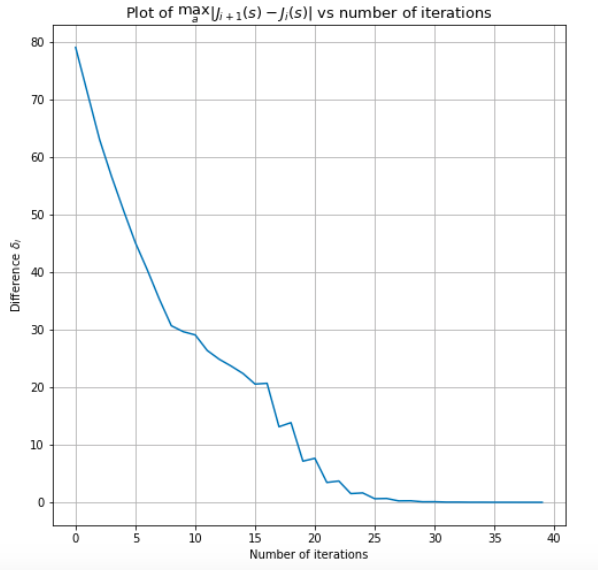
\includegraphics[width=8cm]{J2.png}
\caption{$\max(|J_{i+1}-J_{i}|)$ vs the number of iterations.}
\end{figure}\\
The value of $\delta_i$ goes below the value of 0.01 after 37 iterations. Thus it is ideal to stop the loop after 37 iterations as we have a converged value.


\section{Goal 1:}
 
 \begin{figure}[h]
 \centering
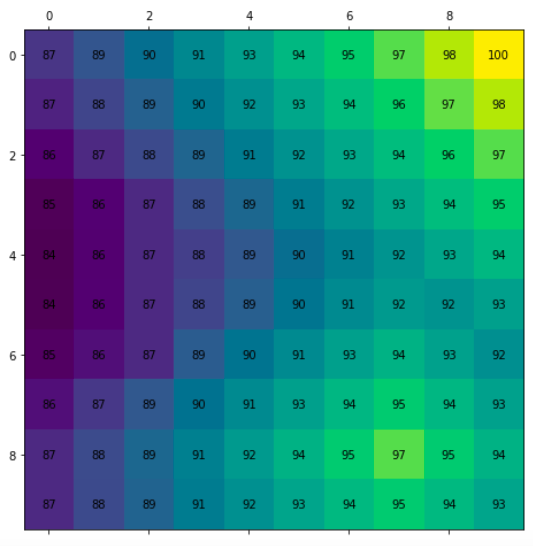
\includegraphics[width=8cm]{J_matrix1.png}
\caption{$J(s)$ after the termination of the loop}
\end{figure}

\begin{figure}[h]
 \centering
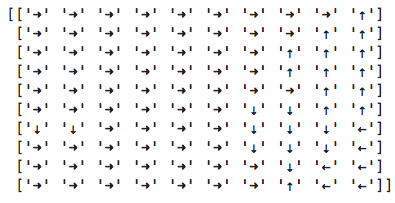
\includegraphics[width=8cm]{Action1.png}
\caption{$\Pi(s)$ after the termination of the loop}
\end{figure}
The rewards can be explained as follows:
\begin{itemize}
\item The reward at the 'gray IN' cell is quite low as it takes us further away from 'GOAL 1'
\item The rewards decreases as we go further away from the 'GOAL 1' (taking into considerations the effects of the wormhole)
\item The rewards at the 'orange IN' cell are higher than it's neighbours because these cells take us closer to the 'GOAL 1'
\end{itemize}
Note: The actions in the 'Goal' cell and the 'IN' cell are not valid as one cannot take action in those cells.

The actions can be explained as follows:
\begin{itemize}
\item The actions around the 'orange IN' cell point into the cell as going into that cell takes to the 'orange OUT' which is nearer to 'GOAL 1' 
\item The actions around the 'GOAL 2' point into the goal which is quite obvious.
\item Starting in any state we will always land up in 'GOAL 1' which means that there are no improper policies.
\end{itemize}



\section{Goal 2:}
 
 \begin{figure}[h]
 \centering
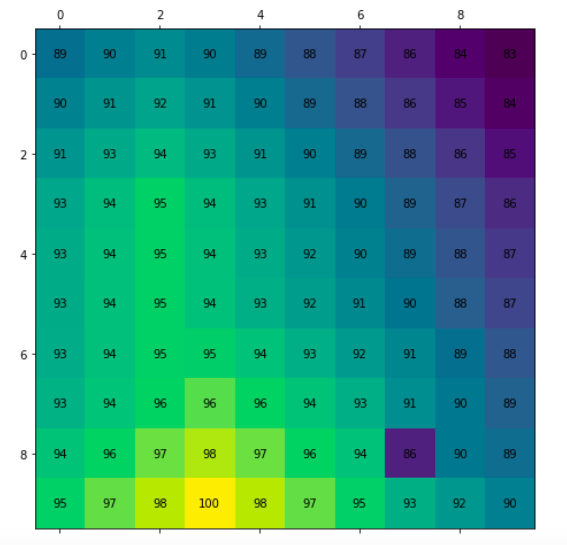
\includegraphics[width=8cm]{J_matrix2.png}
\caption{$J(s)$ after the termination of the loop}
\end{figure}

\begin{figure}[h]
 \centering
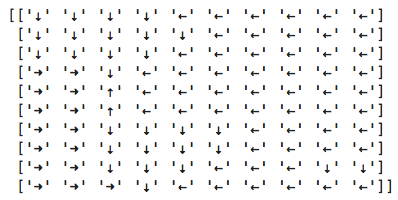
\includegraphics[width=8cm]{Action2.png}
\caption{$\Pi(s)$ after the termination of the loop}
\end{figure}

The rewards can be explained as follows:
\begin{itemize}
\item The reward at the 'orange IN' cell is quite low as it takes us further away from 'GOAL 2'
\item The rewards decreases as we go further away from the 'GOAL 2'
\item The rewards at the 'gray IN' cell are higher than it's neighbours because these cells take us closer to the 'GOAL 2'
\item The reward is lowest at the top right most corner and highest at the 'GOAL 2'
\end{itemize}
Note: The actions in the 'Goal' cell and the 'IN' cell are not valid as one cannot take action in those cells.

The actions can be explained as follows:
\begin{itemize}
\item The actions around the 'orange IN' cell do not point into the cell as going into that cell takes to the 'orange OUT' which is further away from the 'GOAL 2' 
\item The actions around the 'gray IN' cell point towards the 'gray IN' cell as it will takes us to the 'gray OUT' which is near the 'GOAL 2'
\item The actions around the 'GOAL 2' point into the goal which is quite obvious.
\item Starting in any state we will always land up in 'GOAL 2' which means that there are no improper policies.
\end{itemize}

\section{Plots after 10 iterations}
\begin{figure}[h]
 \centering
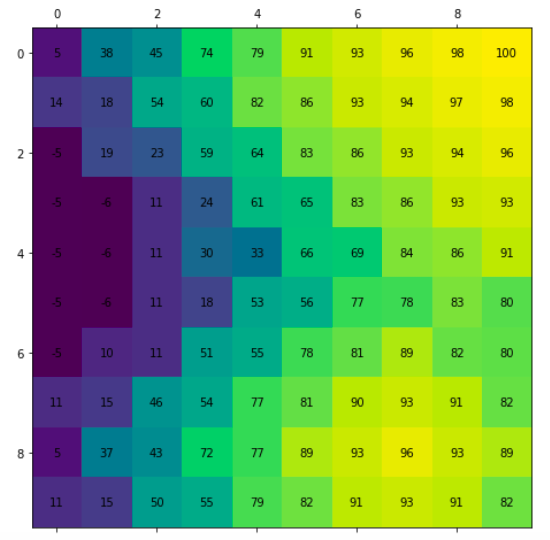
\includegraphics[width=8cm]{J1_10.png}
\caption{$J(s)$ after 10 iterations of the loop for GOAL 1}
\end{figure}

\begin{figure}[h]
 \centering
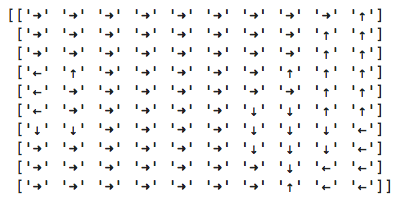
\includegraphics[width=8cm]{Actions_10.png}
\caption{$\Pi(s)$ after 10 iterations of the loop for GOAL 1}
\end{figure}

\begin{figure}[h]
 \centering
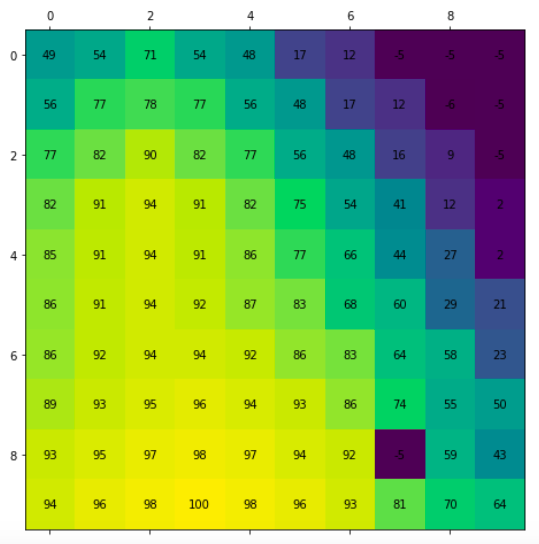
\includegraphics[width=8cm]{J2_10.png}
\caption{$J(s)$ after 10 iterations of the loop for GOAL 2}
\end{figure}

\begin{figure}[h]
 \centering
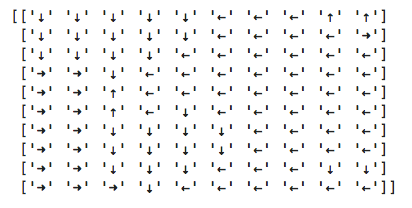
\includegraphics[width=8cm]{Actions_210.png}
\caption{$\Pi(s)$ after 10 iterations of the loop for GOAL 2}
\end{figure}


\section{Plots after 25 iterations}
\begin{figure}[h]
 \centering
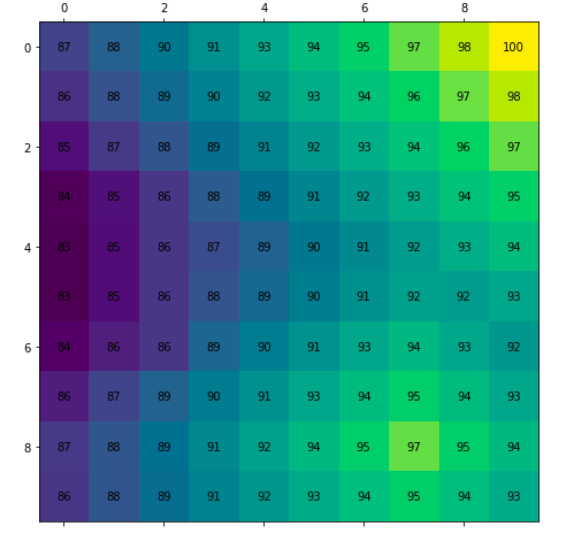
\includegraphics[width=8cm]{J1_25.png}
\caption{$J(s)$ after 25 iterations of the loop for GOAL 1}
\end{figure}

\begin{figure}[h]
 \centering
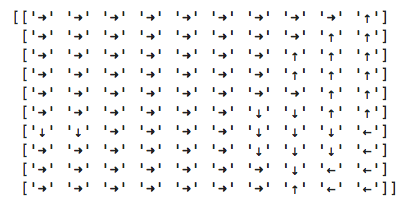
\includegraphics[width=8cm]{Actions_25.png}
\caption{$\Pi(s)$ after 25 iterations of the loop for GOAL 1}
\end{figure}

\begin{figure}[h]
 \centering
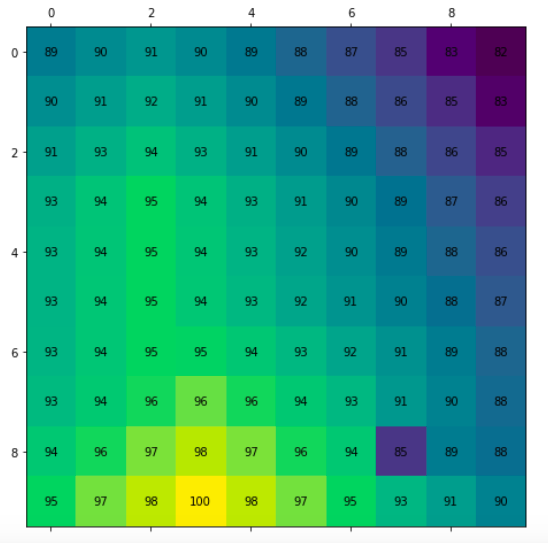
\includegraphics[width=8cm]{J2_25.png}
\caption{$J(s)$ after 25 iterations of the loop for GOAL 2}
\end{figure}

\begin{figure}[h]
 \centering
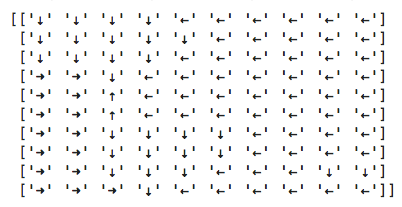
\includegraphics[width=8cm]{Actions_225.png}
\caption{$\Pi(s)$ after 25 iterations of the loop for GOAL 2}
\end{figure}
%%%%%%%%%%%%%%%%%%%%%%%%%%%%%%%%%%%%%%%%%%%%%%%%%%%%%%%%%%%%%%%%%%%%%%%%%%%%%%%%%%%%%%%%%%%%%%%%%%%%%%%%%%%%%%%%%%%%%%
\section{References:}
\begin{itemize}
\item Course Notes
\item Dynamic Programming and Optimal Control by D.Bertsekas.
\end{itemize}










\end{document}
